\documentclass[conference]{IEEEtran}
\IEEEoverridecommandlockouts\usepackage{cite}
\usepackage{amsmath,amssymb,amsfonts}
\usepackage{algorithmic}
\usepackage{graphicx}
\usepackage{textcomp}
\usepackage{xcolor}
\usepackage{array}
\usepackage{enumitem}
\usepackage{siunitx}
\usepackage[spanish]{babel}
\usepackage{multirow}
\usepackage{float}
\usepackage{booktabs}
\usepackage[hidelinks]{hyperref}
\usepackage{hhline}
\usepackage[left=2cm,right=2cm,top=2cm,bottom=2cm]{geometry}
\usepackage{listings}
\usepackage{xcolor}


\lstset{
    language=C,
    basicstyle=\ttfamily\footnotesize,
    frame=single,
    breaklines=true,          % ✅ enable word wrap
    breakatwhitespace=false,  % wrap even in the middle of words if needed
    columns=fullflexible,
    keepspaces=true,
    captionpos=b,
    showstringspaces=false,
    tabsize=4,
    aboveskip=1em,
    belowskip=1em
}

\def\BibTeX{{\rm B\kern-.05em{\sc i\kern-.025em b}\kern-.08em
    T\kern-.1667em\lower.7ex\hbox{E}\kern-.125emX}}
    
\begin{document}

\title{Microcontroladores: Laboratorio 2\\
{\footnotesize \textsuperscript{}
}
\thanks{}
}

\author{\IEEEauthorblockN{1\textsuperscript{st} Hector Pereira}
\IEEEauthorblockA{\textit{Ingeniería en Mecatrónica} \\
\textit{Universidad Tecnológica (UTEC)}\\
Fray Bentos, Uruguay \\
hector.pereira@estudiantes.utec.edu.uy}
\and
\IEEEauthorblockN{2\textsuperscript{nd} Isaac Martirena }
\IEEEauthorblockA{\textit{Ingeniería en Mecatrónica} \\
\textit{Universidad Tecnológica (UTEC)}\\
Fray Bentos, Uruguay \\
isaac.martirena@estudiantes.utec.edu.uy}
}
\maketitle


\begin{abstract}

\end{abstract}

\textit{Keywords: }

\section{Introducción}

% Este laboratorio se enmarca dentro del curso de Microcontroladores, y tiene como objetivo aplicar los conocimientos adquiridos sobre arquitectura AVR y programación en C para el desarrollo de sistemas embebidos funcionales. A diferencia del laboratorio anterior, que se centró en el manejo básico de periféricos y estructuras de control, en esta segunda instancia se busca integrar varios módulos interactivos en un entorno de tiempo real.

\subsection{Propósito del laboratorio}

% El objetivo principal es diseñar, programar e integrar distintos subsistemas sobre el microcontrolador ATmega328P, demostrando el uso combinado de entradas analógicas y digitales, comunicación serial, control por PWM, almacenamiento no volátil y planificación de tareas. Cada módulo implementado aborda un conjunto diferente de competencias, permitiendo comprender el funcionamiento coordinado del hardware y el software en un entorno embebido.

\subsection{Descripción general de los módulos}

% El laboratorio se divide en cuatro desarrollos principales:

    % Plotter: sistema de control cartesiano para movimiento de ejes y trazado de figuras.

    % Colores: sensor RGB con medición por LDR, control de servomotor y replicación visual en una tira LED.

    % Piano: reproducción de melodías mediante timers, interrupciones y manejo de frecuencias.

    % Cerradura electrónica: sistema de acceso con contraseña almacenada en EEPROM, teclado matricial y pantalla LCD.

\subsection{Competencias desarrolladas}

% A través de estos proyectos se ejercitan competencias fundamentales en ingeniería mecatrónica, tales como:

    % Programación estructurada en lenguaje C sobre microcontroladores AVR.

    % Uso de interrupciones y temporizadores para tareas concurrentes.

    % Aplicación de PWM para control de actuadores.

    % Implementación de comunicación serial (USART) y almacenamiento persistente (EEPROM).

    % Diseño de máquinas de estado para gestionar la interacción con el usuario.

\subsection{Cierre o enfoque global}

% En conjunto, el laboratorio permite afianzar la comprensión del funcionamiento interno del ATmega328P y su ecosistema de periféricos, aplicando conceptos de electrónica digital, control en tiempo real y diseño de interfaces. El resultado es un conjunto de sistemas autónomos capaces de procesar información, interactuar con el entorno y ofrecer respuestas predecibles y seguras.

\section{Marco teórico}

\subsection{Procesamiento de señales y sensores de color}

% Explicar brevemente cómo funciona un LDR (Light Dependent Resistor) y su relación entre resistencia e intensidad luminosa.

% Introducir el modelo de color RGB, sus componentes y cómo se representan los colores en un espacio tridimensional.

% Explicar el concepto de calibración y cómo la distancia euclidiana puede emplearse para identificar colores a partir de valores de sensores.

\subsection{Señales PWM y control de servomotores}

% Explicar el principio del PWM (Pulse Width Modulation) y su relación con el control del ángulo en servos.

% Incluir cómo el Timer1 genera una señal PWM con un periodo de 20 ms para mover el servomotor.

\subsection{Reproducción de sonido digital}

% Introducir la relación entre frecuencia y tono musical.

% Explicar cómo los timers generan ondas cuadradas que excitan un buzzer piezoeléctrico.

% Mencionar la noción de melodía digital y uso de estructuras de datos o interrupciones para reproducir secuencias musicales.

\subsection{Interfaz de usuario e interacción hombre–máquina}

% Explicar brevemente qué es una interfaz de usuario (UI) en sistemas embebidos.

% Describir cómo una máquina de estados organiza la interacción entre el usuario y el sistema (teclado, LCD, LEDs, buzzer).

% Introducir la idea de feedback visual y auditivo.

\subsection{Almacenamiento no volátil y EEPROM}

% Describir las características principales de la memoria EEPROM, su capacidad, durabilidad y limitaciones de escritura.

% Explicar su uso para guardar contraseñas o configuraciones persistentes.

\subsection{Planificación temporal y multitarea cooperativa}

% Introducir el concepto de task scheduler o planificador de tareas basado en un contador global (como millis).

% Explicar cómo un solo timer puede manejar varios procesos periódicos sin bloqueos ni polling.

\section{Metodología}

\subsection{Materiales y Herramientas}

\begin{itemize}
    \item Microcontrolador ATmega328P (Arduino Uno)
    \item Sensor LDR y LED RGB
    \item Servomotor SG90
    \item Teclado matricial 4x4
    \item Pantalla LCD 16x2 con interfaz I2C
    \item Buzzers piezoeléctricos (activo y pasivo)
    \item Tira LED WS2812
    \item Resistencias, cables, protoboard
    \item Software: Microchip Studio, Proteus / PicSimLab, Python (para generación de secuencias del plotter)
\end{itemize}

\subsection{Procedimiento general}
Se dividió el sistema en cuatro módulos independientes (Plotter, Colores, Piano y Cerradura).

\subsubsection{\textbf{Plotter}}

    \vspace{1em}
    
\subsubsection{\textbf{Colores}}
    El proceso de reconocimiento de colores se fundamenta en la descomposición de cada color en sus componentes primarias dentro del modelo RGB (\textit{Red}, \textit{Green}, \textit{Blue}). Un color puede representarse como la combinación ponderada de estas tres intensidades, lo que permite su descripción en un espacio tridimensional.  

    \vspace{1em}

    Sin embargo, el sensor fotoresistivo (LDR, \textit{Light Dependent Resistor}) utilizado en el sistema no distingue de forma individual las componentes cromáticas del espectro visible; únicamente mide la intensidad total de luz reflejada sobre su superficie. Si la iluminación se realiza con luz blanca, el sensor solo entrega una lectura proporcional a la cantidad total de luz reflejada, sin discriminar su composición espectral. Este fenómeno equivale a una percepción en escala de grises, dificultando la identificación precisa de colores.

    \vspace{1em}

    Para resolver esta limitación, se empleó un diodo emisor de luz RGB como fuente de iluminación controlada. Al iluminar secuencialmente la superficie con luz roja, verde y azul, el sistema obtiene tres mediciones independientes mediante el LDR. Dichos valores, convertidos por el módulo ADC (\textit{Analog-to-Digital Converter}) del microcontrolador ATmega328P, representan las coordenadas $(R, G, B)$ de un punto dentro de un espacio de color tridimensional.

    \vspace{1em}

    Dado que tanto la respuesta espectral del LDR como la emisión de los LED presentan variaciones no lineales, los valores obtenidos no son directamente proporcionales a las componentes RGB teóricas. No obstante, se implementa un proceso de calibración inicial para contrarrestar estos efectos, donde se miden manualmente los colores de referencia (rojo, verde, azul claro, violeta, morado, amarillo y blanco) y se almacenan sus valores de respeusta RGB de conversión analógica-digital.

    \vspace{1em}

    Cada color de referencia calibrado se modela como un vector fijo en dicho espacio. Para identificar un color, se calcula la distancia euclidiana entre el vector de medición y cada uno de los vectores de referencia almacenados:

    \begin{equation}\label{eq:distancia_color}
    D = \sqrt{(R_m - R_i)^2 + (G_m - G_i)^2 + (B_m - B_i)^2}
    \end{equation}

    donde $(R_m, G_m, B_m)$ representan los valores medidos por el sensor y $(R_i, G_i, B_i)$ corresponden a los valores calibrados de cada color de la hoja de referencia. El color identificado será aquel cuya distancia $D$ sea mínima.

    \vspace{1em}

    El circuito se implementó mediante un divisor resistivo conectado a una de las entradas analógicas del microcontrolador. El color identificado se replica visualmente en la tira de LED WS2812, y el servomotor se posiciona en el ángulo correspondiente (predefinido) al color detectado dentro de la hoja de referencia, integrando así un sistema de selección e identificación de color completamente automatizado.

    \vspace{1em}

\subsubsection{\textbf{Piano}}
    \paragraph*{\textbf{Notas musicales}}---
    El sonido es una onda mecánica que se propaga a través de un medio elástico, producto de variaciones periódicas de presión. Estas ondas pueden clasificarse según su forma en senoidales, cuadradas, triangulares o diente de sierra, dependiendo del patrón temporal de oscilación. En los sistemas digitales, las señales más sencillas de generar son las ondas cuadradas, donde el voltaje alterna entre dos niveles definidos, representando los estados lógicos alto y bajo del microcontrolador.

    \vspace{1em}

    Para producir sonido de manera electrónica, se emplean dispositivos piezoeléctricos denominados \textit{buzzers}. Estos transductores convierten la energía eléctrica en vibraciones mecánicas audibles. Cuando el microcontrolador aplica una señal cuadrada a la entrada del buzzer, el material piezoeléctrico se deforma y contrae periódicamente, generando un sonido cuya frecuencia está directamente relacionada con la frecuencia de la señal de entrada.

    \vspace{1em}

    En el microcontrolador ATmega328P, esta señal se genera mediante el uso de los temporizadores internos (\textit{timers}), configurados para producir una onda cuadrada en un pin de salida. Al modificar la frecuencia de conmutación, es posible variar el tono percibido, ya que la frecuencia del sonido determina su altura musical. De esta manera, cada nota puede asociarse a una frecuencia específica según la escala. Por ejemplo, la nota \textit{La4} corresponde a una frecuencia de 440\,Hz, mientras que \textit{Do4} equivale aproximadamente a 262\,Hz.

    \vspace{1em}

    \paragraph*{\textbf{Reproducir música}}---
    Una nota musical puede representarse computacionalmente mediante tres parámetros fundamentales: la frecuencia de oscilación, la duración temporal durante la cual se mantiene activa y la duración inactiva o en silencio. Cuando el buzzer emite una secuencia ordenada de notas, cada una con su frecuencia, tiempo de activación, y silencio, se obtiene una melodía. En términos programáticos, una melodía se define como un conjunto de estructuras de datos que contienen pares \texttt{(frecuencia, tiempo\_on, tiempo\_off)}, los cuales son procesados secuencialmente para generar la música deseada.
    
    Para crear pistas de canciones se utilizó la herramienta \textit{MIDI to Arduino Converter}~\cite{arduino_midi_converter}, la cual permite convertir pistas MIDI al formato anteriormente mencionado, y almacenarlas dentro de la memoria del microcontrolador.

    \vspace{1em}

    La reproducción simultánea de varios instrumentos en un entorno digital requiere el manejo de múltiples secuencias de notas en paralelo. Para lograrlo sin recurrir al uso de ciclos de espera activos (\textit{polling}), se utilizan interrupciones asociadas a los temporizadores. De este modo, el microcontrolador puede controlar la duración y el inicio de cada nota de forma independiente y precisa, optimizando el uso del procesador y permitiendo la ejecución de tareas concurrentes, como la lectura de entradas o la comunicación serial, mientras la música continúa sonando de manera autónoma.

    \vspace{1em}

    \paragraph*{\textbf{Modo piano}}---
    Para implementar el modo piano se decidió utilizar 8 pulsadores correspondientes a las 8 principales notas musicales. Cada uno de los pulsadores fue conectado a un pin del puerto D del microcontrolador, configurando los pines como entradas y pull-ups internas. Utilizando interrupciones externas por cambio de pin (\texttt{PCINT}) y lógica programática para debouncing, se implementó la funcionalidad de que mientras el pulsador está presionado, la nota sigue sonando.

    \vspace{1em}

    Finalmente, a este sistema se integra funcionalidad USART para mostrar un menú al usuario por consola y permitir comandar el funcionamiento del sistema de manera sencilla. El usuario es presentado con 3 opciones: [1]: Reproducir canción 1, [2]: Reproducir cancion 2, [P]: Cambiar a modo piano. Mediante variables de control se deshabilita la funcionalidad de piano durante la reproducción de canciones, y vice versa, al cambiar al modo piano se detiene y reinician las pistas que se estaban reproduciendo.


    \vspace{1em}

    En síntesis, el sistema desarrollado utiliza un buzzer piezoeléctrico controlado por los temporizadores del ATmega328P para reproducir notas musicales definidas por su frecuencia y duración. A través de la programación de secuencias almacenadas en memoria, es posible interpretar melodías completas y gestionar la reproducción de distintas canciones sin intervención del usuario durante la ejecución. Utilizando USART se puede comandar al programa para reproducir diferentes pistas guardadas o cambiar a modo piano donde 8 pulsadores reproducen las 8 notas principales.

    \vspace{1em}

\subsubsection{\textbf{Cerradura}}
    \paragraph*{\textbf{Funcionamiento general}}---
    El sistema de cerradura electrónica desarrollado tiene como objetivo controlar el acceso mediante una contraseña numérica almacenada en memoria no volátil. Inicialmente, el dispositivo se encuentra en estado de \textit{candado cerrado}. Cuando el usuario ingresa la contraseña correcta, el sistema cambia al estado de \textit{candado abierto}, permitiendo el acceso. En caso de introducir una contraseña incorrecta tres veces consecutivas, se activa una alarma acústica a través de un buzzer, indicando un intento de acceso no autorizado.

    \vspace{1em}

    El sistema también permite modificar la contraseña almacenada. Para ello, el usuario debe ingresar primero la contraseña actual y, tras su validación, definir una nueva contraseña de entre cuatro y seis dígitos. Esta nueva clave se almacena permanentemente en la memoria EEPROM del microcontrolador, garantizando su persistencia incluso después de un apagado o reinicio del sistema.

    \begin{figure}[H]
        \centering
        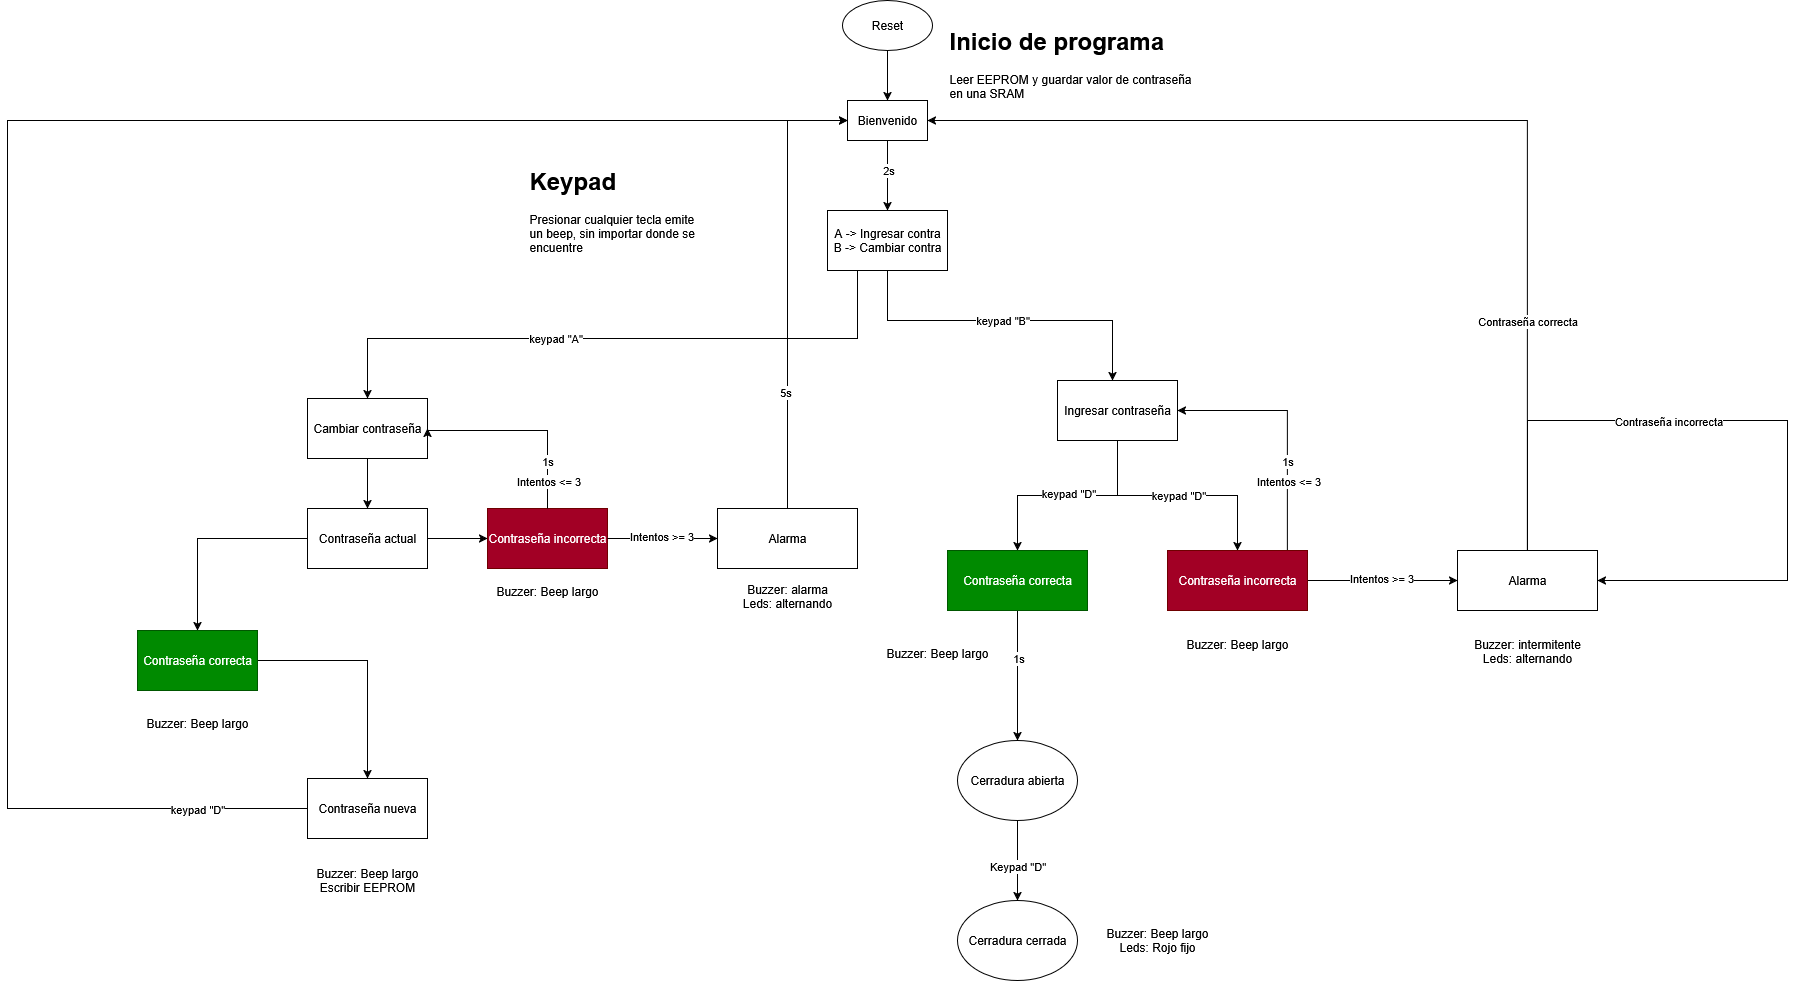
\includegraphics[width=0.9\columnwidth]{anexos/cerradura/DiagramaFlujo.png}
        \caption{Diagrama de flujo de programa de cerradura. Fuente: elaboración própia}
        \label{fig:lcd_ui}
    \end{figure}

    \vspace{1em}
    \paragraph*{\textbf{Interfaz de usuario}}---
    La cerradura dispone de una interfaz de usuario compuesta por una pantalla LCD de 16x2, un teclado matricial 4x4 y tres indicadores luminosos (LED verde, LED rojo y alarma sonora). En este contexto, la interfaz constituye el medio de comunicación entre el usuario y el sistema, mostrando mensajes informativos y recibiendo acciones por medio del teclado. Cada interacción del usuario genera una respuesta visual o acústica distinta, representando así un flujo de diálogo entre ambos.

    \vspace{1em}

    El sistema se diseñó siguiendo una lógica de \textit{máquina de estados finitos}, en la que cada modo de operación (menú principal, ingreso de contraseña, cambio de clave, acceso autorizado, alarma, etc.) representa un estado. Las transiciones entre estados se producen en función de las acciones del usuario y las condiciones del sistema. Este enfoque facilita la gestión de comportamientos complejos, simplifica el control del flujo de ejecución y mejora la legibilidad del código.

    \vspace{1em}
    \paragraph*{\textbf{Teclado matricial}}---
    El ingreso de datos se realiza mediante un teclado matricial 4x4 que combina filas y columnas, optimizando el uso de pines del microcontrolador. Las filas se configuran como salidas y las columnas como entradas con resistencias de \textit{pull-up} activadas. El proceso de lectura consiste en activar una fila a nivel bajo (0) mientras las demás permanecen en alto (1); si alguna tecla de esa fila se encuentra presionada, la columna correspondiente cambia a nivel bajo, permitiendo identificar la intersección entre fila y columna.  

    \vspace{1em}

    Cada tecla se asocia a un carácter según su posición dentro de la matriz, lo que permite retornar el valor numérico o simbólico correspondiente. Para evitar falsas detecciones debido al rebote mecánico de los contactos, se aplica una rutina de \textit{debouncing} por software basada en pequeños retardos temporizados.

    \vspace{1em}

    \paragraph*{\textbf{Planificador de tareas}}---
    Durante el funcionamiento, el sistema debe ejecutar múltiples tareas de forma paralela: reproducción de sonidos, manejo de alarmas, parpadeo de LEDs, lectura del teclado y actualización de la pantalla LCD. Sin embargo, el ATmega328P dispone de un número limitado de temporizadores, por lo que no es posible asignar un temporizador independiente a cada tarea.

    \vspace{1em}

    Para resolver esta limitación, se implementó un esquema de ejecución basado en un \textit{planificador de tareas} o \textit{task scheduler} de propósito general. Se utiliza un solo temporizador configurado para generar interrupciones periódicas, incrementando un contador global de 32 bits que actúa como referencia temporal (en milisegundos). Cada tarea compara el tiempo actual con el instante programado de su próxima ejecución, y si se cumple el intervalo, se ejecuta la acción correspondiente. De este modo, múltiples eventos temporizados pueden coexistir sin emplear retardos bloqueantes ni técnicas de \textit{polling}.

    \vspace{1em}

    Para asegurar que la contraseña permanezca almacenada tras un apagado, se utiliza la memoria EEPROM interna del ATmega328P. Esta memoria no volátil permite conservar los datos durante décadas sin alimentación eléctrica, aunque posee un número limitado de ciclos de escritura (aproximadamente $10^5$ operaciones por celda). Por ello, el sistema únicamente escribe en EEPROM cuando el usuario confirma un cambio de contraseña, minimizando el desgaste de la memoria.

    \vspace{1em}

    La lectura y escritura se realizan mediante las funciones de la biblioteca estándar \texttt{avr/eeprom.h}, que permiten transferir cadenas de caracteres directamente desde y hacia direcciones específicas de la EEPROM. Así, el sistema recupera la contraseña almacenada al inicio del programa y la compara con la ingresada por el usuario durante la operación normal.

    \vspace{1em}

    En conjunto, la cerradura electrónica combina la interacción mediante teclado y pantalla LCD, la gestión de tareas en tiempo real y el almacenamiento persistente de datos, logrando un sistema confiable y autónomo. El uso de una máquina de estados y un planificador temporal basado en un único temporizador permite controlar de manera eficiente múltiples procesos simultáneos sin bloquear la ejecución principal del programa.



\section{Resultados}
\subsection{Plotter}
\subsection{Colores}


El proceso de reconocimiento de colores se fundamenta en la descomposición de cada color en sus componentes primarias dentro del modelo RGB (\textit{Red}, \textit{Green}, \textit{Blue}). Un color puede representarse como la combinación ponderada de estas tres intensidades, lo que permite su descripción en un espacio tridimensional.  

\vspace{1em}

Sin embargo, el sensor fotoresistivo (LDR, \textit{Light Dependent Resistor}) utilizado en el sistema no distingue de forma individual las componentes cromáticas del espectro visible; únicamente mide la intensidad total de luz reflejada sobre su superficie. Si la iluminación se realiza con luz blanca, el sensor solo entrega una lectura proporcional a la cantidad total de luz reflejada, sin discriminar su composición espectral. Este fenómeno equivale a una percepción en escala de grises, dificultando la identificación precisa de colores.

\vspace{1em}

Para resolver esta limitación, se empleó un diodo emisor de luz RGB como fuente de iluminación controlada. Al iluminar secuencialmente la superficie con luz roja, verde y azul, el sistema obtiene tres mediciones independientes mediante el LDR. Dichos valores, convertidos por el módulo ADC (\textit{Analog-to-Digital Converter}) del microcontrolador ATmega328P, representan las coordenadas $(R, G, B)$ de un punto dentro de un espacio de color tridimensional.

\vspace{1em}

Dado que tanto la respuesta espectral del LDR como la emisión de los LED presentan variaciones no lineales, los valores obtenidos no son directamente proporcionales a las componentes RGB teóricas. No obstante, el sistema logra resultados estables mediante un proceso de calibración inicial, donde se iluminan sucesivamente los colores de referencia (rojo, verde, azul claro, violeta, morado, amarillo y blanco) y se almacenan sus valores de conversión analógica-digital.

\vspace{1em}

Cada color de referencia calibrado se modela como un vector fijo en dicho espacio. Para identificar un color, se calcula la distancia euclidiana entre el vector de medición y cada uno de los vectores de referencia almacenados:

\begin{equation}\label{eq:distancia_color}
D = \sqrt{(R_m - R_i)^2 + (G_m - G_i)^2 + (B_m - B_i)^2}
\end{equation}

donde $(R_m, G_m, B_m)$ representan los valores medidos por el sensor y $(R_i, G_i, B_i)$ corresponden a los valores calibrados de cada color de la hoja de referencia. El color identificado será aquel cuya distancia $D$ sea mínima.



\vspace{1em}

El circuito se implementó mediante un divisor resistivo conectado a una de las entradas analógicas del microcontrolador. El color identificado se replica visualmente en la tira de LED WS2812, y el servomotor se posiciona en el ángulo correspondiente al color detectado dentro de la hoja de referencia, integrando así un sistema de selección e identificación de color completamente automatizado.


% Reconocer colores
% Como se reconoce un color
% Un color se puede descomoner en otros colores
% Colores primarios
% Colores CYMK
% Colores RGB
% Un LDR no puede medir componentes
% Un LDR solo mide luz reflejada
% Si iluminamos con luz blanca el LDR mide la cantidad de luz blanca que rebota
% Seria como tener vision en blanco y negro
% Algunos colores serian dificiles de identificar

% Si iluminamos con otro color el LDR ve la cantidad de luz que refleja de ese color
% Si iluminamos con rojo, luego verde, y luego azul el LDR puede identificar 
% colores con 3 grados de libertad como el ojo humano.

% Se utiliza un led RGB para iluminar con estos colores

% El LDR no responde la misma manera a todos los tipos de luz. 
% Los valores medidos no se van a correlacionar de manera directa
% Con las componentes tradicionales de cada color.
% Ademas de que existen variaciones de emision de luz entre los mismos colores del led

% Sin embargo es suficiente si lo calibramos antes

% Utilizando un divisor de voltaje se conecta el ldr a un pin analogico del arduino

% Se ilumina con rojo verde y azul para cada color y se recopilan los valores medidos por el ADC

% Se mapean los 6 colores de la hoja para tomar como referencias.

% Para determinar el color el cual el LDR esta apuntando
% se calcula cual es el valor más próximo tomando
% en cuenta los 3 componentes como ejes de libertad
% realizando un calculo de distancia cartesiana.
% A2 + B2 + C2 = D2

% En este caso rojo verde y azul representan un eje en un espacio tridimensional. 
% Los colores calibrados representan vectores. Y el vector de medición se 
% mueve a lo largo de todo este espacio adquiriendo diferentes valores rgb.

% De manera ciclica se mide la distancia del vector medicion con respecto 
% al resto de vectores mapeados para identificar cual es el vector que 
% mas se aproxima al vector medición

% Problemas
% Como medir colores con presicion
% Como reconocer colores precalibrados
% Como controlar un servomotor
% Como controlar una tira LED

% Funcionaldiades
% Salida de info por USART
% Color indicado por angulo en servomotor
% Color indica








\begin{lstlisting}[language=C, caption={Librerias utilizadas}]
#define F_CPU 16000000UL

#include <avr/io.h>
#include <util/delay.h>
#include <avr/interrupt.h>
#include <string.h>
\end{lstlisting}

\begin{lstlisting}[language=C, caption={Mapeado de colores}]
typedef struct {
	const char *name;
	uint16_t r, g, b;
} ColorRef;

const ColorRef color_refs[] = {
	{"MORADO",    216, 157, 274},
	{"ROJO",       206, 149, 262},
	{"AMARILLO",    196, 99, 105},
	{"VERDE",     272, 192, 152},
	{"AZUL CLARO", 151, 153, 122},
	{"VIOLETA",    253, 275, 338},
	{"BLANCO",    110, 93, 91},
};
\end{lstlisting}

\begin{lstlisting}[language=C, caption={Convertidor de unsigned integer a string}]
// Convierte un valor entero sin signo en un string
void UTOA(uint16_t value, char *buffer) { 
	char temp[6];
	int i = 0, j = 0;

	if (value == 0) {
		buffer[0] = '0';
		buffer[1] = '\0';
		return;
	}

	// Convert digits to temp buffer (reversed)
	while (value > 0 && i < sizeof(temp) - 1) {
		temp[i++] = (value % 10) + '0';
		value /= 10;
	}

	// Reverse digits into final buffer
	while (i > 0) buffer[j++] = temp[--i];
	buffer[j] = '\0';
}
\end{lstlisting}

\begin{lstlisting}[language=C, caption={Enviado de datos a tira LED}]
void send_bit(uint8_t bitVal){
	if(bitVal){
		PORTD |=  (1<<LED_PIN);
		asm volatile (
		"nop\n\t""nop\n\t""nop\n\t""nop\n\t""nop\n\t"
		"nop\n\t""nop\n\t""nop\n\t""nop\n\t");
		
		PORTD &= ~(1<<LED_PIN);
		
		asm volatile (
		"nop\n\t""nop\n\t""nop\n\t""nop\n\t");
		
		} else {
		PORTD |=  (1<<LED_PIN);
		asm volatile (
		"nop\n\t""nop\n\t""nop\n\t");
		
		PORTD &= ~(1<<LED_PIN);
		asm volatile (
		"nop\n\t""nop\n\t""nop\n\t""nop\n\t""nop\n\t"
		"nop\n\t""nop\n\t""nop\n\t""nop\n\t""nop\n\t");
	}
}

// Envia un Byte a la tira de leds
// Utiliza cli y sei para un timing preciso
void send_byte(uint8_t byte) {
	cli();  
	for (uint8_t i = 0; i < 8; i++) {
		send_bit(byte & 0x80);  // send most significant bit first
		byte <<= 1;             // shift next bit into MSB position
	}
	sei();  // re-enable interrupts
}
\end{lstlisting}

\begin{lstlisting}[language=C, caption={Inicializadores}]
void usart_init(void) {
	const uint16_t ubrr = (16000000UL / (16UL * BAUD_RATE)) - 1;
	UBRR0H = ubrr >> 8;
	UBRR0L = ubrr;
	UCSR0A = 0;
	UCSR0B = (1 << TXEN0) | (1 << RXEN0) | (1 << RXCIE0);   // RX interrupt
	UCSR0C = (1 << UCSZ01) | (1 << UCSZ00);               // 8N1
}

void adc_init(void) {
	ADMUX  = (1 << REFS0);                        
	ADCSRA = (1 << ADEN)                          
	| (1 << ADPS2) | (1 << ADPS1) | (1 << ADPS0); // Prescaler 128
}

void rgb_init(void){
	DDRB |= (1<<RED) | (1<<GREEN) | (1<<BLUE);
}


void servo_init(void) {
	SERVO_DDR |= (1 << SERVO_PORT); 

	TCCR1A = (1 << COM1A1) | (1 << WGM11);
	TCCR1B = (1 << WGM13) | (1 << WGM12) | (1 << CS11); // 8

	ICR1 = 39999;   
}
 
void ws2812_init(void) { // tira de leds
	LED_DDR |= (1 << LED_PIN);
}
\end{lstlisting}

\begin{lstlisting}[language=C, caption={Funciones de utilidad}]
void ws2812_send_pixel(uint8_t r, uint8_t g, uint8_t b) {
	// Cambiar orden dependiendo de formato de tira led o matriz
	send_byte(g);
	send_byte(b);
	send_byte(r);
}

// Encender n leds del mismo color
void ws2812_fill(uint8_t r, uint8_t g, uint8_t b, uint16_t n) {
	cli(); 
	for (uint16_t i = 0; i < n; i++) {
		ws2812_send_pixel(r, g, b);
	}
	sei();
	ws2812_show();
}

// Establecer colores predeterminados
void led_strip_set_color(uint8_t color_id) {
	uint8_t r = 0, g = 0, b = 0;

	switch (color_id) {
		case 1: // Rojo
		r = 255; g = 0; b = 0;
		break;

		case 2: // Amarillo
		r = 255; g = 100; b = 0;
		break;

		case 3: // Verde
		r = 0; g = 255; b = 0;
		break;

		case 4: // Azul claro
		r = 0; g = 255; b = 255;
		break;

		case 5: // Violeta
		r = 100; g = 0; b = 100;
		
		break;

		case 6: // Morado
		r = 200; g = 0; b = 75;
		
		break;

		case 7: // Blanco
		r = 255; g = 255; b = 255;
		break;

		default: // Apagar LED
		r = g = b = 0;
		break;
	}

	ws2812_fill(r, g, b, 50);
}

// Establecer angulo en el servomotor
void servo_set_angle(uint8_t angle) {
	uint16_t pulse = 1000 + ((uint32_t)angle * 4000) / 180;
	OCR1A = pulse;
}

// Leer adc
uint16_t adc_read(uint8_t channel) {
	ADMUX = (ADMUX & 0xF0) | (channel & 0x0F);  
	ADCSRA |= (1 << ADSC);                     
	while (ADCSRA & (1 << ADSC));               // Wait for conversion to finish
	return ADC;                                 
}

// Establecer color del led rgb (iluminador)
void rgb_set(uint8_t r, uint8_t g, uint8_t b) {
	PORTB = (PORTB & ~((1 << RED)|(1 << GREEN)|(1 << BLUE))) |
	((r<<RED) | (g<<GREEN) | (b<<BLUE));
}

// Identificar color a partir de valores rgb.
// Tomando cada valor calibrado como un vector, se determina la distancia
// cartesiana del vector leido por el sensor.
const char* identify_color(uint16_t r, uint16_t g, uint16_t b) {
	uint32_t best_dist = 0xFFFFFFFF;
	const char *best_name = "UNKNOWN";

	for (uint8_t i = 0; i < NUM_COLORS; i++) {
		int32_t dr = (int32_t)r - color_refs[i].r;
		int32_t dg = (int32_t)g - color_refs[i].g;
		int32_t db = (int32_t)b - color_refs[i].b;
		uint32_t dist = dr*dr + dg*dg + db*db;

		if (dist < best_dist) {
			best_dist = dist;
			best_name = color_refs[i].name;
		}
	}
	return best_name;
}
\end{lstlisting}


\begin{lstlisting}[language=C, caption={Bucle principal}]
// programa principal
int main(void) {
	ws2812_init();
	usart_init();
	adc_init();
	rgb_init();
	servo_init();
	sei();
	
	while (1) {
		rgb_read();
		_delay_ms(50);

	
	}
}
\end{lstlisting}













\subsection{Piano}

El sonido es una onda mecánica que se propaga a través de un medio elástico, producto de variaciones periódicas de presión. Estas ondas pueden clasificarse según su forma en senoidales, cuadradas, triangulares o diente de sierra, dependiendo del patrón temporal de oscilación. En los sistemas digitales, las señales más sencillas de generar son las ondas cuadradas, donde el voltaje alterna entre dos niveles definidos, representando los estados lógicos alto y bajo del microcontrolador.

\vspace{1em}

Para producir sonido de manera electrónica, se emplean dispositivos piezoeléctricos denominados \textit{buzzers}. Estos transductores convierten la energía eléctrica en vibraciones mecánicas audibles. Cuando el microcontrolador aplica una señal cuadrada a la entrada del buzzer, el material piezoeléctrico se deforma y contrae periódicamente, generando un sonido cuya frecuencia está directamente relacionada con la frecuencia de la señal de entrada.

\vspace{1em}

En el microcontrolador ATmega328P, esta señal se genera mediante el uso de los temporizadores internos (\textit{timers}), configurados para producir una onda cuadrada en un pin de salida. Al modificar la frecuencia de conmutación, es posible variar el tono percibido, ya que la frecuencia del sonido determina su altura musical. De esta manera, cada nota puede asociarse a una frecuencia específica según la escala temperada. Por ejemplo, la nota \textit{La4} corresponde a una frecuencia de 440\,Hz, mientras que \textit{Do4} equivale aproximadamente a 262\,Hz.

\vspace{1em}

Una nota musical puede representarse computacionalmente mediante dos parámetros fundamentales: la frecuencia de oscilación, la duración temporal durante la cual se mantiene activa y la duración inactiva o en silencio. Cuando el buzzer emite una secuencia ordenada de notas, cada una con su tiempo de activación y silencio, se obtiene una melodía. En términos programáticos, una melodía se define como un conjunto de estructuras de datos que contienen pares \texttt{(frecuencia, tiempo\_on, tiempo\_off)}, los cuales son procesados secuencialmente para generar la música deseada.

\vspace{1em}

La reproducción simultánea de varios instrumentos en un entorno digital requiere el manejo de múltiples secuencias de notas en paralelo. Para lograrlo sin recurrir al uso de ciclos de espera activos (\textit{polling}), se utilizan interrupciones asociadas a los temporizadores. De este modo, el microcontrolador puede controlar la duración y el inicio de cada nota de forma independiente y precisa, optimizando el uso del procesador y permitiendo la ejecución de tareas concurrentes, como la lectura de entradas o la comunicación serial, mientras la música continúa sonando de manera autónoma.

\vspace{1em}

En síntesis, el sistema desarrollado utiliza un buzzer piezoeléctrico controlado por los temporizadores del ATmega328P para reproducir notas musicales definidas por su frecuencia y duración. A través de la programación de secuencias almacenadas en memoria, es posible interpretar melodías completas y gestionar la reproducción de distintas canciones sin intervención del usuario durante la ejecución.



% Sonido
% Que es el sonido
% Ondas
% Difrentes tipos de ondas
% Como hacemos sonido
% Buzzer
% Onda cuadrada
% Como funciona el buzzer
% Piezo
% Como lo hacemos sonar con el atmega
% Variacion de frecuencia
% Como hacemos otro sonido
% Cambiamos la frencuencia
% Como hacemos musica
% Teoria musical basica
% Mapeo de notas
% Una nota es una frecuencia
% Una frecuencia durante un tiempo es una nota
% Como guardamos musica
% Nota musical: frencuencia, tiempo encendido, tiempo apagado
% Secuencia de notas musicales --- musica
% La musica se compone de varios instrumentos en paralelo
% Como reproducimos varios instrumentos
% Evitar polling --- Utilizar timers

% Problemas
% Como reproducir sonido
% Como representar una nota musical
% Como reproducir pistas en paralelo

% Funcionalidades
% Control por USART
% Piano fisico


USART con buffers
\begin{lstlisting}[language=C, caption={Funciones USART con buffering}]

#define TX_BUF_SZ 128
#define TX_MASK   (TX_BUF_SZ - 1)

#define RX_BUF_SZ 128
#define RX_MASK   (RX_BUF_SZ - 1)

uint8_t tx_buf[TX_BUF_SZ];
uint8_t tx_head = 0, tx_tail = 0;

uint8_t rx_buf[RX_BUF_SZ];
uint8_t rx_head = 0, rx_tail = 0;

uint8_t usart_rx_available(void) {
	return (uint8_t)((rx_head - rx_tail) & RX_MASK);
}

void usart_init_9600(void) {
	const uint16_t ubrr = (16000000UL / (16UL * 9600)) - 1;
	UBRR0H = ubrr >> 8;
	UBRR0L = ubrr;
	UCSR0A = 0;
	UCSR0B = _BV(TXEN0) | _BV(RXEN0) | _BV(RXCIE0);   // <- RX interrupt
	UCSR0C = _BV(UCSZ01) | _BV(UCSZ00);               // 8N1
}

// USART
void usart_init_9600(void) {
	const uint16_t ubrr = (16000000UL / (16UL * 9600)) - 1;
	UBRR0H = ubrr >> 8;
	UBRR0L = ubrr;
	UCSR0A = 0;
	UCSR0B = _BV(TXEN0) | _BV(RXEN0) | _BV(RXCIE0);   // <- RX interrupt
	UCSR0C = _BV(UCSZ01) | _BV(UCSZ00);               // 8N1
}

// Escribir byte al buffer
uint8_t usart_write_try(uint8_t b) {
	uint8_t next = (uint8_t)((tx_head + 1) & TX_MASK);
	if (next == tx_tail) return 0;               // buffer lleno
	tx_buf[tx_head] = b;
	tx_head = next;
	UCSR0B |= _BV(UDRIE0);                       // kick the ISR
	return 1;
}

// Escribir string al buffer
uint16_t usart_write_str(const char *s) {
	uint16_t n = 0;
	while (*s && usart_write_try((uint8_t)*s++)) n++;
	return n;
}

// Leer byte del buffer de recepcion
uint8_t usart_read_try(uint8_t *b) {
	if (rx_head == rx_tail) return 0;                
	*b = rx_buf[rx_tail];
	rx_tail = (uint8_t)((rx_tail + 1) & RX_MASK);
	return 1;
}

// Interrupcion de registro de TX libre
ISR(USART_UDRE_vect) {
	if (tx_head == tx_tail) {                    
		UCSR0B &= (uint8_t)~_BV(UDRIE0);         
		return;
	}
	UDR0 = tx_buf[tx_tail];
	tx_tail = (uint8_t)((tx_tail + 1) & TX_MASK);
}

// Interrupcion de dato recibido
ISR(USART_RX_vect) {
	uint8_t d = UDR0;
	uint8_t next = (uint8_t)((rx_head + 1) & RX_MASK);
	if (next != rx_tail) {                
		rx_buf[rx_head] = d;
		rx_head = next;
	}
}
\end{lstlisting}

Formato de guardado de canciones
\begin{lstlisting}[language=C, caption={Guardado de canciones}]
// Midi tracks
// Generated using https://github.com/ShivamJoker/MIDI-to-Arduino
const int midiC[827][3] PROGMEM = {
	{E5, 94, 0},
	{B4, 94, 0},
	{A4, 94, 0},
	{E4, 94, 0},
	{A4, 94, 0},
	{B4, 94, 0}
    // ... 
}
\end{lstlisting}

\begin{lstlisting}[language=C, caption={Manejo de eventos RX USART}]
void handleUSART(uint8_t character){
	if (character == '1'){
		mode = 1;
		eventAoff = 1;
		eventBoff = 0;
		
		song = 0;
		
		eventAon = 0; // Encender track A
		indexA = 0; // Posicion track A
		countA = 0; // Conteo de overflow de notas de track A
		maxCountAon = 0; // Maximo conteo de overflow encendido en A
		maxCountAoff = 0; // Maximo conteo de overflow apagado en A
		enableCountAon = 0; // Habilitar conteo de encendido en A
		enableCountAoff = 0; // Habilidad conteo de apagado en A
		
		eventBon = 0; // Encender track B
		indexB = 0; // Posicion track B
		countB = 0; // Conteo de overflow de notas de track B
		maxCountBon = 0; // Maximo conteo de overflow encendido en B
		maxCountBoff = 0; // Maximo conteo de overflow apagado en B
		enableCountBon = 0; // Habilitar conteo de encendido en B
		enableCountBoff = 0; // Habilidad conteo de apagado en B
		
		PCICR &= ~((1 << PCIE1) | (1 << PCIE2));
		stopFrequencyB();
		
	} else if (character == '2'){
		mode = 1;
		eventAoff = 1;
		eventBoff = 1;
		
		song = 1;
		
		eventAon = 0; // Encender track A
		indexA = 0; // Posicion track A
		countA = 0; // Conteo de overflow de notas de track A
		maxCountAon = 0; // Maximo conteo de overflow encendido en A
		maxCountAoff = 0; // Maximo conteo de overflow apagado en A
		enableCountAon = 0; // Habilitar conteo de encendido en A
		enableCountAoff = 0; // Habilidad conteo de apagado en A
		
		eventBon = 0; // Encender track B
		indexB = 0; // Posicion track B
		countB = 0; // Conteo de overflow de notas de track B
		maxCountBon = 0; // Maximo conteo de overflow encendido en B
		maxCountBoff = 0; // Maximo conteo de overflow apagado en B
		enableCountBon = 0; // Habilitar conteo de encendido en B
		enableCountBoff = 0; // Habilidad conteo de apagado en B
		
		PCICR &= ~((1 << PCIE1) | (1 << PCIE2));
		stopFrequencyA();

	} else if (character == 'P'){
		mode = 0;
		eventAoff = 0;
		eventBoff = 0;
				
		eventAon = 0; // Encender track A
		indexA = 0; // Posicion track A
		countA = 0; // Conteo de overflow de notas de track A
		maxCountAon = 0; // Maximo conteo de overflow encendido en A
		maxCountAoff = 0; // Maximo conteo de overflow apagado en A
		enableCountAon = 0; // Habilitar conteo de encendido en A
		enableCountAoff = 0; // Habilidad conteo de apagado en A
				
		eventBon = 0; // Encender track B
		indexB = 0; // Posicion track B
		countB = 0; // Conteo de overflow de notas de track B
		maxCountBon = 0; // Maximo conteo de overflow encendido en B
		maxCountBoff = 0; // Maximo conteo de overflow apagado en B
		enableCountBon = 0; // Habilitar conteo de encendido en B
		enableCountBoff = 0; // Habilidad conteo de apagado en B
		
		startDebounceTimer();
		stopFrequencyA();
		stopFrequencyB();
	}
}
\end{lstlisting}


\begin{lstlisting}[language=C, caption={Reproduccion de frecuencias}]
void playFrequencyA(uint16_t freq) {
	if (!freq) return;  

	DDRD |= (1 << PORTD6);
	
	// Elegir prescaler adecuado para esa frecuencia

	uint8_t presc_bits = 0;     
	uint16_t ocr = 0;

	const uint16_t presc_list[] = {8, 64, 256, 1024};
	const uint8_t  bits_list[]  = {0b010, 0b011, 0b100, 0b101};

	for (uint8_t i = 0; i < 4; i++) {
		ocr = (F_CPU / (2UL * presc_list[i] * freq)) - 1;
		if (ocr <= 255) {
			presc_bits = bits_list[i];
			break;
		}
	}

	TCCR0A = (1 << COM0A0) | (1 << WGM01);
	TCCR0B = presc_bits;          
	OCR0A  = (uint8_t)ocr;        
}
\end{lstlisting}





\begin{lstlisting}[language=C, caption={Variables de control de flujo}]
uint8_t eventAon = 0; // Encender track A
uint8_t eventAoff = 0; // Apagar track A
uint16_t indexA = 0; // Posicion track A
uint16_t countA = 0; // Conteo de overflow de notas de A
uint16_t maxCountAon = 0; // Maximo conteo de overflow encendido en A
uint16_t maxCountAoff = 0; // Maximo conteo de overflow apagado en A
uint8_t enableCountAon = 0; // Habilitar conteo de encendido en A
uint8_t enableCountAoff = 0; // Habilidad conteo de apagado en A

uint8_t eventBon = 0; // Encender track B
uint8_t eventBoff = 0; // Apagar track B
uint16_t indexB = 0; // Posicion track B
uint16_t countB = 0; // Conteo de overflow de notas de B
uint16_t maxCountBon = 0; // Maximo conteo de overflow encendido en B
uint16_t maxCountBoff = 0; // Maximo conteo de overflow apagado en B
uint8_t enableCountBon = 0; // Habilitar conteo encendido en B
uint8_t enableCountBoff = 0; // Habilitar conteo apagado en B
\end{lstlisting}

\begin{lstlisting}[language=C, caption={Variables de control de flujo}]
int main(void) {
	timer1_init();
	usart_init_9600();
	init_piano_buttons();
	sei();
	
	usart_write_str("Elija una opcion:\r\n");
	usart_write_str("[1] Dragon Ball - Cha-La Head-Cha-La\r\n");
	usart_write_str("[2] Portal - Still alive\r\n");
	usart_write_str("[P] Modo piano\r\n");

	
	while (1){
		if (mode == 0){
			piano_mode();
		} else if (mode == 1){
			song_mode();
		}
	    uint8_t c;
	    if (usart_read_try(&c)) {
		    handleUSART(c);
	    }
	}
}
\end{lstlisting}



\subsection{Cerradura}

El sistema de cerradura electrónica desarrollado tiene como objetivo controlar el acceso mediante una contraseña numérica almacenada en memoria no volátil. Inicialmente, el dispositivo se encuentra en estado de \textit{candado cerrado}. Cuando el usuario ingresa la contraseña correcta, el sistema cambia al estado de \textit{candado abierto}, permitiendo el acceso. En caso de introducir una contraseña incorrecta tres veces consecutivas, se activa una alarma acústica a través de un buzzer, indicando un intento de acceso no autorizado.

El sistema también permite modificar la contraseña almacenada. Para ello, el usuario debe ingresar primero la contraseña actual y, tras su validación, definir una nueva contraseña de entre cuatro y seis dígitos. Esta nueva clave se almacena permanentemente en la memoria EEPROM del microcontrolador, garantizando su persistencia incluso después de un apagado o reinicio del sistema.

\vspace{1em}

\subsubsection{Interfaz de usuario e interacción}

La cerradura dispone de una interfaz de usuario compuesta por una pantalla LCD de 16x2, un teclado matricial 4x4 y tres indicadores luminosos (LED verde, LED rojo y alarma sonora). En este contexto, la interfaz constituye el medio de comunicación entre el usuario y el sistema, mostrando mensajes informativos y recibiendo acciones por medio del teclado. Cada interacción del usuario genera una respuesta visual o acústica distinta, representando así un flujo de diálogo entre ambos.

El sistema se diseñó siguiendo una lógica de \textit{máquina de estados finitos}, en la que cada modo de operación (menú principal, ingreso de contraseña, cambio de clave, acceso autorizado, alarma, etc.) representa un estado. Las transiciones entre estados se producen en función de las acciones del usuario y las condiciones del sistema. Este enfoque facilita la gestión de comportamientos complejos, simplifica el control del flujo de ejecución y mejora la legibilidad del código.

\vspace{1em}

\subsubsection{Teclado matricial y detección de teclas}

El ingreso de datos se realiza mediante un teclado matricial 4x4 que combina filas y columnas, optimizando el uso de pines del microcontrolador. Las filas se configuran como salidas y las columnas como entradas con resistencias de \textit{pull-up} activadas. El proceso de lectura consiste en activar una fila a nivel bajo (0) mientras las demás permanecen en alto (1); si alguna tecla de esa fila se encuentra presionada, la columna correspondiente cambia a nivel bajo, permitiendo identificar la intersección entre fila y columna.  

Cada tecla se asocia a un carácter según su posición dentro de la matriz, lo que permite retornar el valor numérico o simbólico correspondiente. Para evitar falsas detecciones debido al rebote mecánico de los contactos, se aplica una rutina de \textit{debouncing} por software basada en pequeños retardos temporizados.

\vspace{1em}

\subsubsection{Gestión temporal y concurrencia de tareas}

Durante el funcionamiento, el sistema debe ejecutar múltiples tareas de forma paralela: reproducción de sonidos, manejo de alarmas, parpadeo de LEDs, lectura del teclado y actualización de la pantalla LCD. Sin embargo, el ATmega328P dispone de un número limitado de temporizadores, por lo que no es posible asignar un temporizador independiente a cada tarea.

Para resolver esta limitación, se implementó un esquema de ejecución basado en un \textit{planificador de tareas} o \textit{task scheduler} de propósito general. Se utiliza un solo temporizador configurado para generar interrupciones periódicas, incrementando un contador global de 32 bits que actúa como referencia temporal (en milisegundos). Cada tarea compara el tiempo actual con el instante programado de su próxima ejecución, y si se cumple el intervalo, se ejecuta la acción correspondiente. De este modo, múltiples eventos temporizados pueden coexistir sin emplear retardos bloqueantes ni técnicas de \textit{polling}.

\vspace{1em}

\subsubsection{Almacenamiento persistente de la contraseña}

Para asegurar que la contraseña permanezca almacenada tras un apagado, se utiliza la memoria EEPROM interna del ATmega328P. Esta memoria no volátil permite conservar los datos durante décadas sin alimentación eléctrica, aunque posee un número limitado de ciclos de escritura (aproximadamente $10^5$ operaciones por celda). Por ello, el sistema únicamente escribe en EEPROM cuando el usuario confirma un cambio de contraseña, minimizando el desgaste de la memoria.

La lectura y escritura se realizan mediante las funciones de la biblioteca estándar \texttt{avr/eeprom.h}, que permiten transferir cadenas de caracteres directamente desde y hacia direcciones específicas de la EEPROM. Así, el sistema recupera la contraseña almacenada al inicio del programa y la compara con la ingresada por el usuario durante la operación normal.

\vspace{1em}

\subsubsection{Resumen de funcionamiento}

En conjunto, la cerradura electrónica combina la interacción mediante teclado y pantalla LCD, la gestión de tareas en tiempo real y el almacenamiento persistente de datos, logrando un sistema confiable y autónomo. El uso de una máquina de estados y un planificador temporal basado en un único temporizador permite controlar de manera eficiente múltiples procesos simultáneos sin bloquear la ejecución principal del programa.


% Cerradura
% Que tiene que hacer
% Candado cerrado
% Contraseña correcta
% Candado abierto
% Sino 3 veces alarma

% Cambiar contraseña
% Contra actual
% Contra nueva
% Guaradado

% Contraseñas tienen que ser entre 4 y 6 digitos

% Problema
% Una interfaz de usuario
% Que es una interfaz
% Entradas y salidas
% El usuario hace algo y la interfaz muestra algo
% Es la parte del programa o sistema que se encarga
% de hablar con el usuario.
% Diferentes acciones muestran o hacen diferentes cosas
% Maquina de estados --- Transiciones de estado.
% Problema: Reproducir sonidos, hacer debouncing, manejar alarmas, pantalla LCD. 
% No existen suficientes timers
% Solucion: tareas o tasks
% Utilizar un contador de tiempo interno de 32 bits
% junto con un solo timer para manejar tareas en paralelo

% La tarea se ejecuta rapidamente en el main y compara el timepo que paso con 
% el tiempo especificado para una acción especifica.

% Un solo timer. Muchos delays sin polling.

% Otro problema
% Contraseña debe ser guardada aunque el sistema esté apagado
% Solucion EEPROM
% Funcionamiento de la eeprom
% limitaciones de escritura de EEPROM
% Como leer
% Como escribir

% Otro problema
% Teclado matricial
% Usa menos pines, uno por fila uno por columna
% Como identificar botones presionados
% Respuesta multiplexado
% Filas funcionan como salidas
% Columnas funcionan como entradas (pullup interno)
% Al solamente apagar una fila a la vez (0) 
% va a hacer que el pin de esa columna se vuelva 0
% Funcion retorna el caracter que representa esa fila y columna
% Listo.



Diagrama de Flujo

\begin{figure}[H]
    \centering
    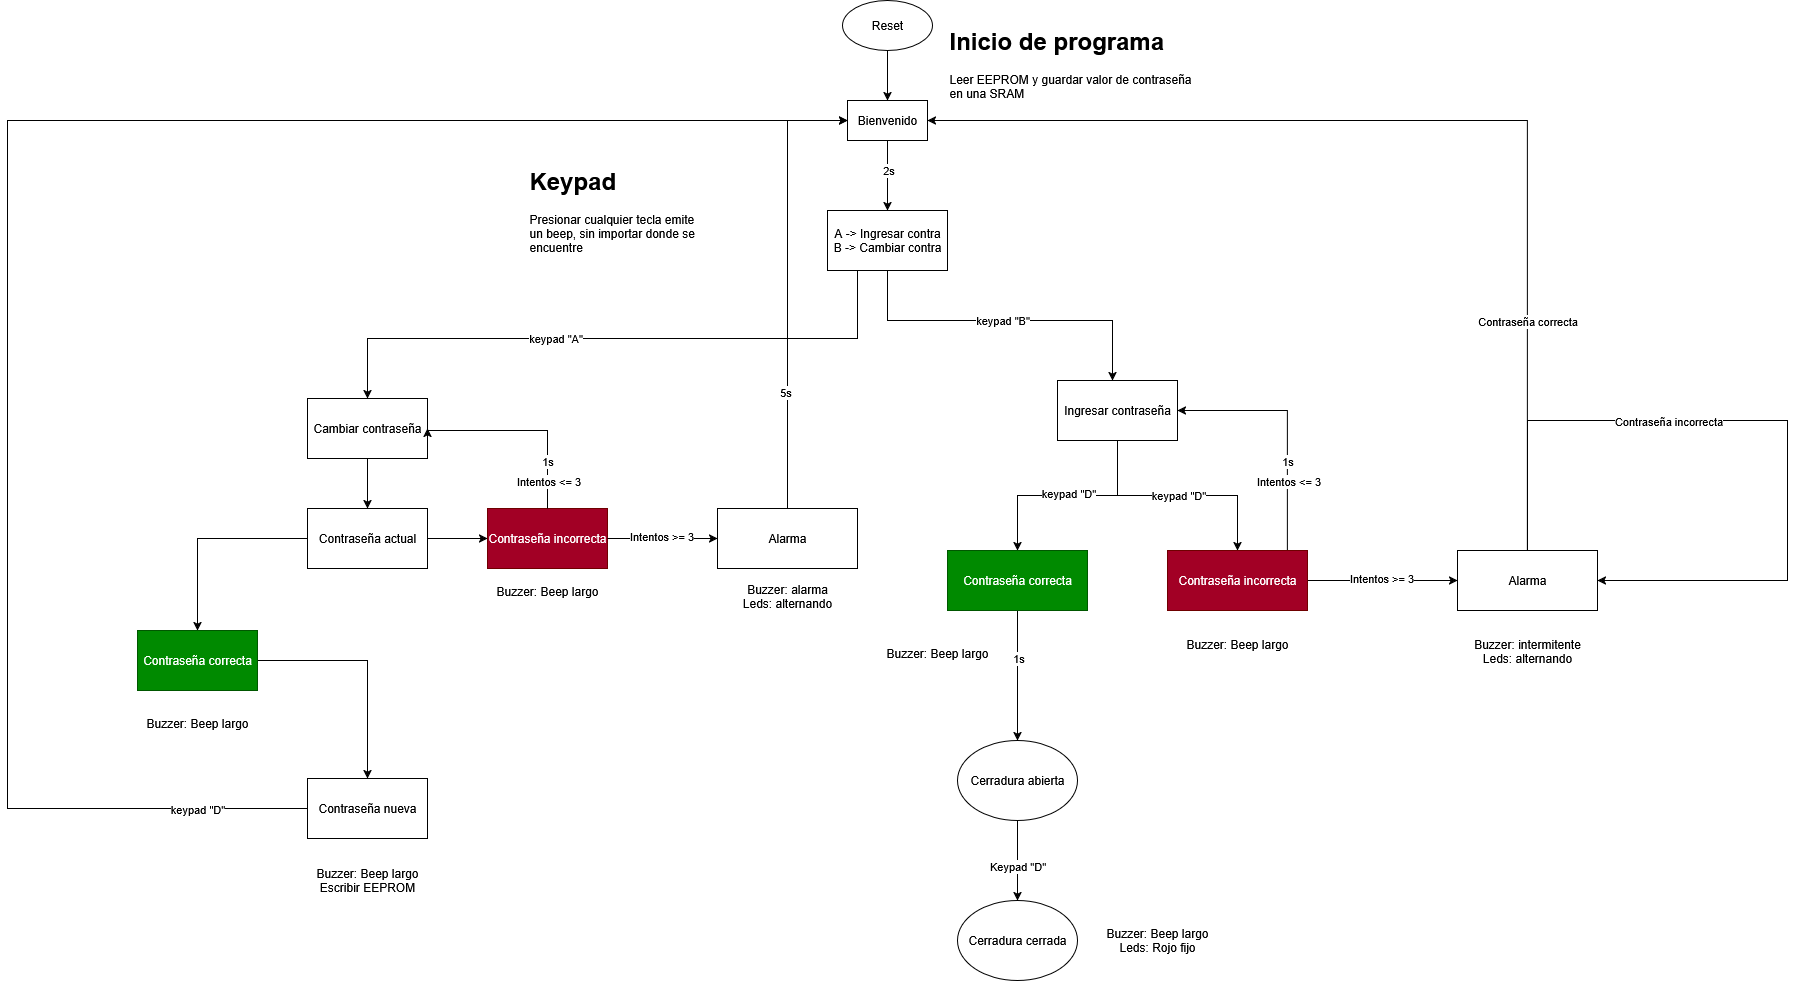
\includegraphics[width=0.9\columnwidth]{anexos/cerradura/DiagramaFlujo.png}
    \caption{Diagrama de flujo. Fuente: elaboración própia}
    \label{fig:lcd_ui}
\end{figure}


Librerias para lcd
\begin{lstlisting}[language=C, caption={Librerias utilizadas para pantalla LCD}]
#include "i2c_master.h"
#include "i2c_master.c"
#include "liquid_crystal_i2c.h"
#include "liquid_crystal_i2c.c"

int main(void){
    LiquidCrystalDevice_t device = lq_init(0x27, 16, 2, LCD_5x8DOTS);
    lq_turnOnBacklight(&device);
	char welcomeText[] = "Bienvenido!";
	lq_print(&device, welcomeText);
    while (1);
}
\end{lstlisting}


Implementacion de tareas
\begin{lstlisting}[language=C, caption={Implementacion de tareas}]
uint32_t millis_counter = 0;

// Mapeo de keypad
const char keypad[4][4] = {
	{'1', '2', '3', 'A'},
	{'4', '5', '6', 'B'},
	{'7', '8', '9', 'C'},
	{'*', '0', '#', 'D'}
};


uint32_t keypad_on_at = 0;
uint8_t keypad_enable = 1;

ISR(TIMER0_OVF_vect){
    millis_counter++;
}

uint32_t millis_now(void) {
    uint32_t m;
    cli();     // disable interrupts
    m = millis_counter;
    sei();     // re-enable
    return m;
}

void keypad_debounce_ms(uint16_t delay_ms){
    keypad_enable = 0;
    keypad_on_at = millis_now() + delay_ms;
}

void keypad_task(void){
    if (!keypad_enable && (millis_now() > keypad_on_at)){
        keypad_enable = 1;
    }
}   

int main(void){
    // main code ...
    while (1){
        keypad_task();
        // loop code ...
    }
}
\end{lstlisting}

Lectura multiplexada de keypad
\begin{lstlisting}[language=C, caption={Funcion de lectura multiplexada de keypad}]
char keypad_scan(void) {
	if (!keypad_enable) return 0;
	
	uint8_t row, col;
	uint8_t cols;
	static uint8_t prevKey; // store for later

	for (row = 0; row < 4; row++) {
		PORTD = (PORTD | 0xF0) & ~(1 << (row + 4));
		_delay_us(5);  
		cols = PIND & 0x0F;  

		for (col = 0; col < 4; col++) {
			if (!(cols & (1 << col)) ) {
				if ((prevKey == keypad[row][col])) return 0;
				
				keypad_debounce_ms(200);
				prevKey = keypad[row][col];
				return keypad[row][col];  
			} 
		}
	}
	prevKey = 0;
	return 0; 
}
\end{lstlisting}

Tarea de alarma
\begin{lstlisting}[language=C, caption={Tarea de alarma}]
 void alarm_task(void){
	if (!alarm_active) return;
	uint32_t now = millis_now();
	
	if (now > alarm_until){
		alarm_active = 0;
		PORTB &= ~(1<<PORTB5);
		led_red_on();
		return;
	}
	
	if (now > alarm_next_toggle){
		alarm_next_toggle = now + ALARM_TOGGLE_MS;
		if (alarm_phase){
			led_red_on();
		} else {
			led_green_on();
		}
		alarm_phase ^= 1;
		
		buzzer_beep(100);
	}
}
\end{lstlisting}

Escritura y lectura de EEPROM
\begin{lstlisting}[language=C, caption={Escritura y lectura de EEPROM}]
#include <avr/eeprom.h>

#define MAX_PASSWORD_LENGTH 6

#define EEPROM_MAGIC 0x42
uint8_t EEMEM ee_magic;                         // init marker

char storedPassword[MAX_PASSWORD_LENGTH + 1] = "123456";
char typedPassword[MAX_PASSWORD_LENGTH + 1];

char EEMEM ee_password[MAX_PASSWORD_LENGTH + 1];

void eeprom_load_password(void) {
	uint8_t magic = eeprom_read_byte(&ee_magic);
	if (magic == EEPROM_MAGIC) {
		eeprom_read_block(storedPassword, 
						  ee_password, 
						  MAX_PASSWORD_LENGTH + 1);

		storedPassword[MAX_PASSWORD_LENGTH] = '\0';
		} else {

		eeprom_update_block(storedPassword, ee_password, MAX_PASSWORD_LENGTH + 1);
		eeprom_update_byte(&ee_magic, EEPROM_MAGIC);
	}
	storedPassword_length = strlen(storedPassword);
}

void eeprom_save_password(const char *pwd) {
	
	char temp[MAX_PASSWORD_LENGTH + 1];
	strncpy(temp, pwd, MAX_PASSWORD_LENGTH);
	temp[MAX_PASSWORD_LENGTH] = '\0';
	eeprom_update_block(temp, ee_password, MAX_PASSWORD_LENGTH + 1);
	eeprom_update_byte(&ee_magic, EEPROM_MAGIC);
}
\end{lstlisting}


Logica de estados
\begin{lstlisting}[language=C, caption={Logica de estados}]
typedef enum { UI_MENU, UI_INGRESO, UI_CAMBIO_ACTUAL, UI_CAMBIO_NUEVA, UI_ABIERTO, UI_ALARMA } ui_state_t;

int main(void){
    while(1){
        char key = keypad_scan();
		if (key) {
			switch (ui_state)
			{
                case UI_MENU: break;
                case UI_INGRESO: break;
                case UI_CAMBIO_ACTUAL: break;
                case UI_CAMBIO_NUEVA: break;
                case UI_CAMBIO_ALARMA: break;
                case UI_CAMBIO_ABIERTO: break;
    }
}
\end{lstlisting}








\section{Conlusiones}

\subsection{Plotter}
\subsection{Colores}

\begin{itemize}
\item La comunicación por USART fue una limitación para la velocidad del sistema. Podría mejorarse reduciendo la cantidad de datos enviados o usando interrupciones para hacerlo más fluido.
\item Sería útil agregar un modo de calibración donde el usuario pueda registrar los valores de referencia de cada color, adaptando el sistema a distintas condiciones de luz.
\item Se podría usar un servomotor de 360° para aprovechar todos los colores disponibles en la rueda.
\end{itemize}

\subsection{Piano}

\begin{itemize}
\item Sería interesante agregar más canciones al repertorio.
\item Se podría mejorar la coordinación entre las pistas, ya que con el tiempo tienden a desfasarse un poco.
\item También sería bueno incluir más notas en el teclado para ampliar el rango musical.
\end{itemize}

\subsection{Cerradura}

\begin{itemize}
\item Agregar un botón para ver la contraseña escrita antes de confirmar ayudaría al usuario sin afectar la seguridad.
\item Implementar un solenoide real permitiría que el sistema abra y cierre físicamente el cerrojo.
\item En la simulación de PicSimLab el reinicio no siempre funciona correctamente. A veces es necesario usar el botón “DEBUG” o reiniciar el programa. Sin embargo, en el dispositivo real el sistema funciona correctamente.
\end{itemize}
            
\bibliographystyle{IEEEtran}
\nocite{*}
\bibliography{5_referencias}

\section{Anexos}

\subsection{Fragmentos de codigo}

\subsubsection{Plotter}---

\subsubsection{Colores}---

\begin{lstlisting}[language=C, caption={Librerias utilizadas}]
#define F_CPU 16000000UL

#include <avr/io.h>
#include <util/delay.h>
#include <avr/interrupt.h>
#include <string.h>
\end{lstlisting}

\begin{lstlisting}[language=C, caption={Mapeado de colores}]
typedef struct {
	const char *name;
	uint16_t r, g, b;
} ColorRef;

const ColorRef color_refs[] = {
	{"MORADO",    216, 157, 274},
	{"ROJO",       206, 149, 262},
	{"AMARILLO",    196, 99, 105},
	{"VERDE",     272, 192, 152},
	{"AZUL CLARO", 151, 153, 122},
	{"VIOLETA",    253, 275, 338},
	{"BLANCO",    110, 93, 91},
};
\end{lstlisting}

\begin{lstlisting}[language=C, caption={Convertidor de unsigned integer a string}]
// Convierte un valor entero sin signo en un string
void UTOA(uint16_t value, char *buffer) { 
	char temp[6];
	int i = 0, j = 0;

	if (value == 0) {
		buffer[0] = '0';
		buffer[1] = '\0';
		return;
	}

	// Convert digits to temp buffer (reversed)
	while (value > 0 && i < sizeof(temp) - 1) {
		temp[i++] = (value % 10) + '0';
		value /= 10;
	}

	// Reverse digits into final buffer
	while (i > 0) buffer[j++] = temp[--i];
	buffer[j] = '\0';
}
\end{lstlisting}

\begin{lstlisting}[language=C, caption={Enviado de datos a tira LED}]
void send_bit(uint8_t bitVal){
	if(bitVal){
		PORTD |=  (1<<LED_PIN);
		asm volatile (
		"nop\n\t""nop\n\t""nop\n\t""nop\n\t""nop\n\t"
		"nop\n\t""nop\n\t""nop\n\t""nop\n\t");
		
		PORTD &= ~(1<<LED_PIN);
		
		asm volatile (
		"nop\n\t""nop\n\t""nop\n\t""nop\n\t");
		
		} else {
		PORTD |=  (1<<LED_PIN);
		asm volatile (
		"nop\n\t""nop\n\t""nop\n\t");
		
		PORTD &= ~(1<<LED_PIN);
		asm volatile (
		"nop\n\t""nop\n\t""nop\n\t""nop\n\t""nop\n\t"
		"nop\n\t""nop\n\t""nop\n\t""nop\n\t""nop\n\t");
	}
}

// Envia un Byte a la tira de leds
// Utiliza cli y sei para un timing preciso
void send_byte(uint8_t byte) {
	cli();  
	for (uint8_t i = 0; i < 8; i++) {
		send_bit(byte & 0x80);  // send most significant bit first
		byte <<= 1;             // shift next bit into MSB position
	}
	sei();  // re-enable interrupts
}
\end{lstlisting}

\begin{lstlisting}[language=C, caption={Inicializadores}]
void usart_init(void) {
	const uint16_t ubrr = (16000000UL / (16UL * BAUD_RATE)) - 1;
	UBRR0H = ubrr >> 8;
	UBRR0L = ubrr;
	UCSR0A = 0;
	UCSR0B = (1 << TXEN0) | (1 << RXEN0) | (1 << RXCIE0);   // RX interrupt
	UCSR0C = (1 << UCSZ01) | (1 << UCSZ00);               // 8N1
}

void adc_init(void) {
	ADMUX  = (1 << REFS0);                        
	ADCSRA = (1 << ADEN)                          
	| (1 << ADPS2) | (1 << ADPS1) | (1 << ADPS0); // Prescaler 128
}

void rgb_init(void){
	DDRB |= (1<<RED) | (1<<GREEN) | (1<<BLUE);
}


void servo_init(void) {
	SERVO_DDR |= (1 << SERVO_PORT); 

	TCCR1A = (1 << COM1A1) | (1 << WGM11);
	TCCR1B = (1 << WGM13) | (1 << WGM12) | (1 << CS11); // 8

	ICR1 = 39999;   
}
 
void ws2812_init(void) { // tira de leds
	LED_DDR |= (1 << LED_PIN);
}
\end{lstlisting}

\begin{lstlisting}[language=C, caption={Funciones de utilidad}]
void ws2812_send_pixel(uint8_t r, uint8_t g, uint8_t b) {
	// Cambiar orden dependiendo de formato de tira led o matriz
	send_byte(g);
	send_byte(b);
	send_byte(r);
}

// Encender n leds del mismo color
void ws2812_fill(uint8_t r, uint8_t g, uint8_t b, uint16_t n) {
	cli(); 
	for (uint16_t i = 0; i < n; i++) {
		ws2812_send_pixel(r, g, b);
	}
	sei();
	ws2812_show();
}

// Establecer colores predeterminados
void led_strip_set_color(uint8_t color_id) {
	uint8_t r = 0, g = 0, b = 0;

	switch (color_id) {
		case 1: // Rojo
		r = 255; g = 0; b = 0;
		break;

		case 2: // Amarillo
		r = 255; g = 100; b = 0;
		break;

		case 3: // Verde
		r = 0; g = 255; b = 0;
		break;

		case 4: // Azul claro
		r = 0; g = 255; b = 255;
		break;

		case 5: // Violeta
		r = 100; g = 0; b = 100;
		
		break;

		case 6: // Morado
		r = 200; g = 0; b = 75;
		
		break;

		case 7: // Blanco
		r = 255; g = 255; b = 255;
		break;

		default: // Apagar LED
		r = g = b = 0;
		break;
	}

	ws2812_fill(r, g, b, 50);
}

// Establecer angulo en el servomotor
void servo_set_angle(uint8_t angle) {
	uint16_t pulse = 1000 + ((uint32_t)angle * 4000) / 180;
	OCR1A = pulse;
}

// Leer adc
uint16_t adc_read(uint8_t channel) {
	ADMUX = (ADMUX & 0xF0) | (channel & 0x0F);  
	ADCSRA |= (1 << ADSC);                     
	while (ADCSRA & (1 << ADSC));               // Wait for conversion to finish
	return ADC;                                 
}

// Establecer color del led rgb (iluminador)
void rgb_set(uint8_t r, uint8_t g, uint8_t b) {
	PORTB = (PORTB & ~((1 << RED)|(1 << GREEN)|(1 << BLUE))) |
	((r<<RED) | (g<<GREEN) | (b<<BLUE));
}

// Identificar color a partir de valores rgb.
// Tomando cada valor calibrado como un vector, se determina la distancia
// cartesiana del vector leido por el sensor.
const char* identify_color(uint16_t r, uint16_t g, uint16_t b) {
	uint32_t best_dist = 0xFFFFFFFF;
	const char *best_name = "UNKNOWN";

	for (uint8_t i = 0; i < NUM_COLORS; i++) {
		int32_t dr = (int32_t)r - color_refs[i].r;
		int32_t dg = (int32_t)g - color_refs[i].g;
		int32_t db = (int32_t)b - color_refs[i].b;
		uint32_t dist = dr*dr + dg*dg + db*db;

		if (dist < best_dist) {
			best_dist = dist;
			best_name = color_refs[i].name;
		}
	}
	return best_name;
}
\end{lstlisting}


\begin{lstlisting}[language=C, caption={Bucle principal}]
// programa principal
int main(void) {
	ws2812_init();
	usart_init();
	adc_init();
	rgb_init();
	servo_init();
	sei();
	
	while (1) {
		rgb_read();
		_delay_ms(50);

	
	}
}
\end{lstlisting}

\subsubsection{Piano}---


USART con buffers
\begin{lstlisting}[language=C, caption={Funciones USART con buffering}]

#define TX_BUF_SZ 128
#define TX_MASK   (TX_BUF_SZ - 1)

#define RX_BUF_SZ 128
#define RX_MASK   (RX_BUF_SZ - 1)

uint8_t tx_buf[TX_BUF_SZ];
uint8_t tx_head = 0, tx_tail = 0;

uint8_t rx_buf[RX_BUF_SZ];
uint8_t rx_head = 0, rx_tail = 0;

uint8_t usart_rx_available(void) {
	return (uint8_t)((rx_head - rx_tail) & RX_MASK);
}

void usart_init_9600(void) {
	const uint16_t ubrr = (16000000UL / (16UL * 9600)) - 1;
	UBRR0H = ubrr >> 8;
	UBRR0L = ubrr;
	UCSR0A = 0;
	UCSR0B = _BV(TXEN0) | _BV(RXEN0) | _BV(RXCIE0);   // <- RX interrupt
	UCSR0C = _BV(UCSZ01) | _BV(UCSZ00);               // 8N1
}

// USART
void usart_init_9600(void) {
	const uint16_t ubrr = (16000000UL / (16UL * 9600)) - 1;
	UBRR0H = ubrr >> 8;
	UBRR0L = ubrr;
	UCSR0A = 0;
	UCSR0B = _BV(TXEN0) | _BV(RXEN0) | _BV(RXCIE0);   // <- RX interrupt
	UCSR0C = _BV(UCSZ01) | _BV(UCSZ00);               // 8N1
}

// Escribir byte al buffer
uint8_t usart_write_try(uint8_t b) {
	uint8_t next = (uint8_t)((tx_head + 1) & TX_MASK);
	if (next == tx_tail) return 0;               // buffer lleno
	tx_buf[tx_head] = b;
	tx_head = next;
	UCSR0B |= _BV(UDRIE0);                       // kick the ISR
	return 1;
}

// Escribir string al buffer
uint16_t usart_write_str(const char *s) {
	uint16_t n = 0;
	while (*s && usart_write_try((uint8_t)*s++)) n++;
	return n;
}

// Leer byte del buffer de recepcion
uint8_t usart_read_try(uint8_t *b) {
	if (rx_head == rx_tail) return 0;                
	*b = rx_buf[rx_tail];
	rx_tail = (uint8_t)((rx_tail + 1) & RX_MASK);
	return 1;
}

// Interrupcion de registro de TX libre
ISR(USART_UDRE_vect) {
	if (tx_head == tx_tail) {                    
		UCSR0B &= (uint8_t)~_BV(UDRIE0);         
		return;
	}
	UDR0 = tx_buf[tx_tail];
	tx_tail = (uint8_t)((tx_tail + 1) & TX_MASK);
}

// Interrupcion de dato recibido
ISR(USART_RX_vect) {
	uint8_t d = UDR0;
	uint8_t next = (uint8_t)((rx_head + 1) & RX_MASK);
	if (next != rx_tail) {                
		rx_buf[rx_head] = d;
		rx_head = next;
	}
}
\end{lstlisting}

Formato de guardado de canciones
\begin{lstlisting}[language=C, caption={Guardado de canciones}]
// Midi tracks
// Generated using https://github.com/ShivamJoker/MIDI-to-Arduino
const int midiC[827][3] PROGMEM = {
	{E5, 94, 0},
	{B4, 94, 0},
	{A4, 94, 0},
	{E4, 94, 0},
	{A4, 94, 0},
	{B4, 94, 0}
    // ... 
}
\end{lstlisting}

\begin{lstlisting}[language=C, caption={Manejo de eventos RX USART}]
void handleUSART(uint8_t character){
	if (character == '1'){
		mode = 1;
		eventAoff = 1;
		eventBoff = 0;
		
		song = 0;
		
		eventAon = 0; // Encender track A
		indexA = 0; // Posicion track A
		countA = 0; // Conteo de overflow de notas de track A
		maxCountAon = 0; // Maximo conteo de overflow encendido en A
		maxCountAoff = 0; // Maximo conteo de overflow apagado en A
		enableCountAon = 0; // Habilitar conteo de encendido en A
		enableCountAoff = 0; // Habilidad conteo de apagado en A
		
		eventBon = 0; // Encender track B
		indexB = 0; // Posicion track B
		countB = 0; // Conteo de overflow de notas de track B
		maxCountBon = 0; // Maximo conteo de overflow encendido en B
		maxCountBoff = 0; // Maximo conteo de overflow apagado en B
		enableCountBon = 0; // Habilitar conteo de encendido en B
		enableCountBoff = 0; // Habilidad conteo de apagado en B
		
		PCICR &= ~((1 << PCIE1) | (1 << PCIE2));
		stopFrequencyB();
		
	} else if (character == '2'){
		mode = 1;
		eventAoff = 1;
		eventBoff = 1;
		
		song = 1;
		
		eventAon = 0; // Encender track A
		indexA = 0; // Posicion track A
		countA = 0; // Conteo de overflow de notas de track A
		maxCountAon = 0; // Maximo conteo de overflow encendido en A
		maxCountAoff = 0; // Maximo conteo de overflow apagado en A
		enableCountAon = 0; // Habilitar conteo de encendido en A
		enableCountAoff = 0; // Habilidad conteo de apagado en A
		
		eventBon = 0; // Encender track B
		indexB = 0; // Posicion track B
		countB = 0; // Conteo de overflow de notas de track B
		maxCountBon = 0; // Maximo conteo de overflow encendido en B
		maxCountBoff = 0; // Maximo conteo de overflow apagado en B
		enableCountBon = 0; // Habilitar conteo de encendido en B
		enableCountBoff = 0; // Habilidad conteo de apagado en B
		
		PCICR &= ~((1 << PCIE1) | (1 << PCIE2));
		stopFrequencyA();

	} else if (character == 'P'){
		mode = 0;
		eventAoff = 0;
		eventBoff = 0;
				
		eventAon = 0; // Encender track A
		indexA = 0; // Posicion track A
		countA = 0; // Conteo de overflow de notas de track A
		maxCountAon = 0; // Maximo conteo de overflow encendido en A
		maxCountAoff = 0; // Maximo conteo de overflow apagado en A
		enableCountAon = 0; // Habilitar conteo de encendido en A
		enableCountAoff = 0; // Habilidad conteo de apagado en A
				
		eventBon = 0; // Encender track B
		indexB = 0; // Posicion track B
		countB = 0; // Conteo de overflow de notas de track B
		maxCountBon = 0; // Maximo conteo de overflow encendido en B
		maxCountBoff = 0; // Maximo conteo de overflow apagado en B
		enableCountBon = 0; // Habilitar conteo de encendido en B
		enableCountBoff = 0; // Habilidad conteo de apagado en B
		
		startDebounceTimer();
		stopFrequencyA();
		stopFrequencyB();
	}
}
\end{lstlisting}


\begin{lstlisting}[language=C, caption={Reproduccion de frecuencias}]
void playFrequencyA(uint16_t freq) {
	if (!freq) return;  

	DDRD |= (1 << PORTD6);
	
	// Elegir prescaler adecuado para esa frecuencia

	uint8_t presc_bits = 0;     
	uint16_t ocr = 0;

	const uint16_t presc_list[] = {8, 64, 256, 1024};
	const uint8_t  bits_list[]  = {0b010, 0b011, 0b100, 0b101};

	for (uint8_t i = 0; i < 4; i++) {
		ocr = (F_CPU / (2UL * presc_list[i] * freq)) - 1;
		if (ocr <= 255) {
			presc_bits = bits_list[i];
			break;
		}
	}

	TCCR0A = (1 << COM0A0) | (1 << WGM01);
	TCCR0B = presc_bits;          
	OCR0A  = (uint8_t)ocr;        
}
\end{lstlisting}





\begin{lstlisting}[language=C, caption={Variables de control de flujo}]
uint8_t eventAon = 0; // Encender track A
uint8_t eventAoff = 0; // Apagar track A
uint16_t indexA = 0; // Posicion track A
uint16_t countA = 0; // Conteo de overflow de notas de A
uint16_t maxCountAon = 0; // Maximo conteo de overflow encendido en A
uint16_t maxCountAoff = 0; // Maximo conteo de overflow apagado en A
uint8_t enableCountAon = 0; // Habilitar conteo de encendido en A
uint8_t enableCountAoff = 0; // Habilidad conteo de apagado en A

uint8_t eventBon = 0; // Encender track B
uint8_t eventBoff = 0; // Apagar track B
uint16_t indexB = 0; // Posicion track B
uint16_t countB = 0; // Conteo de overflow de notas de B
uint16_t maxCountBon = 0; // Maximo conteo de overflow encendido en B
uint16_t maxCountBoff = 0; // Maximo conteo de overflow apagado en B
uint8_t enableCountBon = 0; // Habilitar conteo encendido en B
uint8_t enableCountBoff = 0; // Habilitar conteo apagado en B
\end{lstlisting}

\begin{lstlisting}[language=C, caption={Variables de control de flujo}]
int main(void) {
	timer1_init();
	usart_init_9600();
	init_piano_buttons();
	sei();
	
	usart_write_str("Elija una opcion:\r\n");
	
	usart_write_str(
		"[1] Dragon Ball - Cha-La Head-Cha-La\r\n"
		);

	usart_write_str(
		"[2] Portal - Still alive\r\n"
		);

	usart_write_str("[P] Modo piano\r\n");

	
	while (1){
		if (mode == 0){
			piano_mode();
		} else if (mode == 1){
			song_mode();
		}
	    uint8_t c;
	    if (usart_read_try(&c)) {
		    handleUSART(c);
	    }
	}
}
\end{lstlisting}

\subsubsection{Cerradura}---

Diagrama de Flujo

\begin{figure}[H]
    \centering
    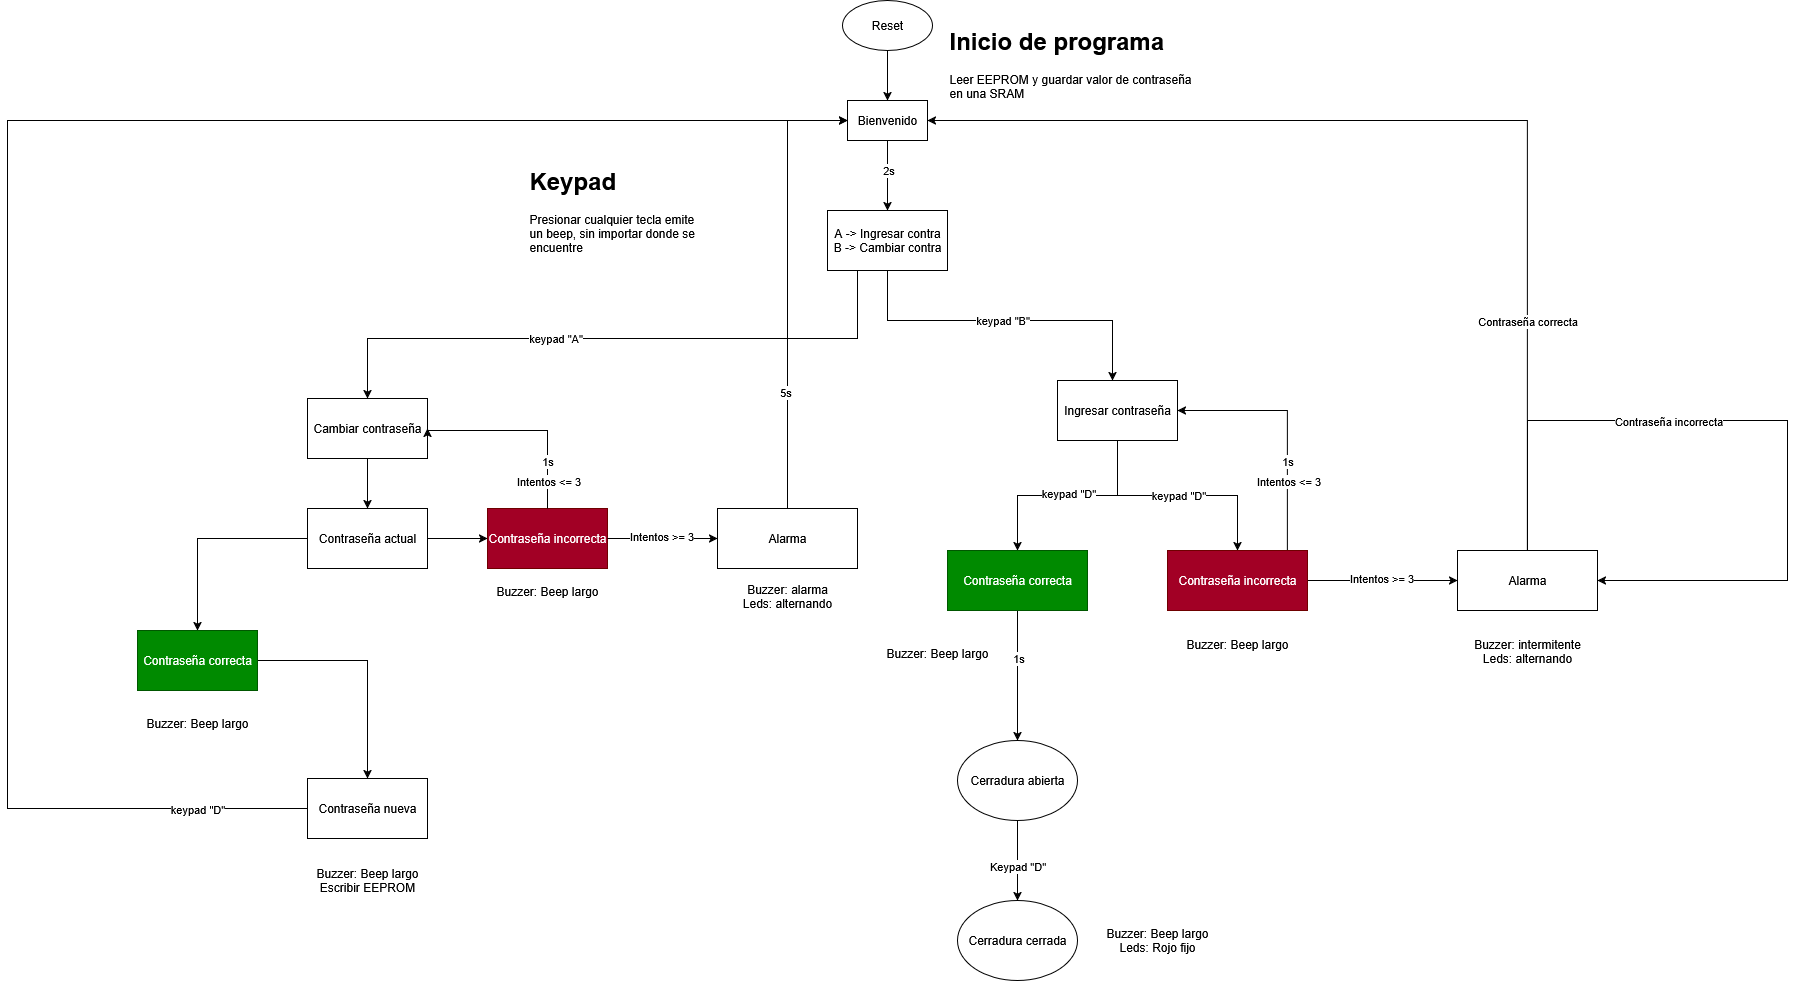
\includegraphics[width=0.9\columnwidth]{anexos/cerradura/DiagramaFlujo.png}
    \caption{Diagrama de flujo. Fuente: elaboración própia}
    \label{fig:lcd_ui}
\end{figure}


Librerias para lcd
\begin{lstlisting}[language=C, caption={Librerias utilizadas para pantalla LCD}]
#include "i2c_master.h"
#include "i2c_master.c"
#include "liquid_crystal_i2c.h"
#include "liquid_crystal_i2c.c"

int main(void){
    LiquidCrystalDevice_t device = lq_init(0x27, 16, 2, LCD_5x8DOTS);
    lq_turnOnBacklight(&device);
	char welcomeText[] = "Bienvenido!";
	lq_print(&device, welcomeText);
    while (1);
}
\end{lstlisting}


Implementacion de tareas
\begin{lstlisting}[language=C, caption={Implementacion de tareas}]
uint32_t millis_counter = 0;

// Mapeo de keypad
const char keypad[4][4] = {
	{'1', '2', '3', 'A'},
	{'4', '5', '6', 'B'},
	{'7', '8', '9', 'C'},
	{'*', '0', '#', 'D'}
};


uint32_t keypad_on_at = 0;
uint8_t keypad_enable = 1;

ISR(TIMER0_OVF_vect){
    millis_counter++;
}

uint32_t millis_now(void) {
    uint32_t m;
    cli();     // disable interrupts
    m = millis_counter;
    sei();     // re-enable
    return m;
}

void keypad_debounce_ms(uint16_t delay_ms){
    keypad_enable = 0;
    keypad_on_at = millis_now() + delay_ms;
}

void keypad_task(void){
    if (!keypad_enable && (millis_now() > keypad_on_at)){
        keypad_enable = 1;
    }
}   

int main(void){
    // main code ...
    while (1){
        keypad_task();
        // loop code ...
    }
}
\end{lstlisting}

Lectura multiplexada de keypad
\begin{lstlisting}[language=C, caption={Funcion de lectura multiplexada de keypad}]
char keypad_scan(void) {
	if (!keypad_enable) return 0;
	
	uint8_t row, col;
	uint8_t cols;
	static uint8_t prevKey; // store for later

	for (row = 0; row < 4; row++) {
		PORTD = (PORTD | 0xF0) & ~(1 << (row + 4));
		_delay_us(5);  
		cols = PIND & 0x0F;  

		for (col = 0; col < 4; col++) {
			if (!(cols & (1 << col)) ) {
				if ((prevKey == keypad[row][col])) return 0;
				
				keypad_debounce_ms(200);
				prevKey = keypad[row][col];
				return keypad[row][col];  
			} 
		}
	}
	prevKey = 0;
	return 0; 
}
\end{lstlisting}

Tarea de alarma
\begin{lstlisting}[language=C, caption={Tarea de alarma}]
 void alarm_task(void){
	if (!alarm_active) return;
	uint32_t now = millis_now();
	
	if (now > alarm_until){
		alarm_active = 0;
		PORTB &= ~(1<<PORTB5);
		led_red_on();
		return;
	}
	
	if (now > alarm_next_toggle){
		alarm_next_toggle = now + ALARM_TOGGLE_MS;
		if (alarm_phase){
			led_red_on();
		} else {
			led_green_on();
		}
		alarm_phase ^= 1;
		
		buzzer_beep(100);
	}
}
\end{lstlisting}

Escritura y lectura de EEPROM
\begin{lstlisting}[language=C, caption={Escritura y lectura de EEPROM}]
#include <avr/eeprom.h>

#define MAX_PASSWORD_LENGTH 6
#define EEPROM_MAGIC 0x42

uint8_t EEMEM ee_magic;                
char EEMEM ee_password[MAX_PASSWORD_LENGTH + 1];

char storedPassword[MAX_PASSWORD_LENGTH + 1] = "123456";
char typedPassword[MAX_PASSWORD_LENGTH + 1];


void eeprom_load_password(void) {
	if (eeprom_read_byte(&ee_magic) != EEPROM_MAGIC) {
		
	eeprom_update_block(
			storedPassword, 
			ee_password, 
			sizeof(storedPassword)
		);

		eeprom_update_byte(&ee_magic, EEPROM_MAGIC);
		} else {
		eeprom_read_block(
			storedPassword, 
			ee_password, 
			sizeof(storedPassword)
		);
	}
}

void eeprom_save_password(const char *pwd) {
	char buf[MAX_PASSWORD_LENGTH + 1];
	strncpy(buf, pwd, MAX_PASSWORD_LENGTH);
	buf[MAX_PASSWORD_LENGTH] = '\0';
	eeprom_update_block(buf, ee_password, sizeof(buf));
}
\end{lstlisting}


Logica de estados
\begin{lstlisting}[language=C, caption={Logica de estados}]
typedef enum { UI_MENU, UI_INGRESO, UI_CAMBIO_ACTUAL, UI_CAMBIO_NUEVA, UI_ABIERTO, UI_ALARMA } ui_state_t;

int main(void){
    while(1){
        char key = keypad_scan();
		if (key) {
			switch (ui_state)
			{
                case UI_MENU: break;
                case UI_INGRESO: break;
                case UI_CAMBIO_ACTUAL: break;
                case UI_CAMBIO_NUEVA: break;
                case UI_CAMBIO_ALARMA: break;
                case UI_CAMBIO_ABIERTO: break;
    }
}
\end{lstlisting}



\end{document}